\chapter{Dataset Building}
\label{cha:4}

\section{BAT dataset}

\subsection{Characteristics} \label{bat-characteristics}

The BAT dataset \cite{spinde-2023-bat} is chosen instead of NLPCSS \cite{chen-etal-2020-nlpcss} for this project due to its article-level suitability and labels fluidity, as well additional metadata as it contains outlets information. It contains 6345 rows of manually labeled news articles from 255 English-speaking news outlets (US-based), originally scraped from Ad Fontes Media's website along with their respective \textbf{political bias} and \textbf{reliability scores}. Articles in the dataset encompassed a wide arrange of topics such as COVID-19, politics, and lifestyle. The political bias score measures the extent of political influence, ranging from -42 (most extreme left) to +42 (most extreme right). The reliability score reflects the article's truthfulness, with values ranging from 0 (least reliable, containing inaccurate or fabricated information) to 64 (most reliable, original fact reporting).

Both political bias and reliability scores on each article were rated using defined metrics and multiple sub-factors, performed by three randomly selected analysts from Ad Fontes Media's team of over 60 experts. The corresponding three scores were then averaged, producing the final article scores. Moreover, each group consists analysts with different beliefs in the political spectrum i.e., left, center, and right.

The reliability score evaluates original fact reporting to analysis, opinion, propaganda, and inaccurate/fabricated information, with scores above 40 generally considered good and scores below 24 typically seen as problematic, scores between 24 and 40 suggest a variety of factors, including a strong presence of opinion and analysis or significant variability in reliability across different articles \cite{adfontes}. This metric is chosen as the main label in this project due to its correlation with textual-level bias: phrasing bias, spin bias, and statement bias described in \ref{media-bias-definition}

\subsection{Extension}

The original BAT dataset only contains news titles and links (along with other metadata) and is missing the body content of articles. To overcome this, a Python script is written and executed, iteratively visiting each of the URL from the dataset and scrape the news content. This was not an easy task as each website has its own unique structures and formats. Furthermore, the scraped text contains noises that are almost impossible to remove through the script. Some outlets such as The Nation, Chicago Tribune, and Truthout required manual intervention as the scraped text were duplicated over themselves. The current extended dataset contains 5270 rows of articles, mainly due to unavailable websites and missing articles.

To remove noises from article content, the text are then pre-processed extensively. All the content of every article in the dataset were joined into one single list, split into words, and then compared against an English word list (cite), resulting in a list of faulty words sorted by their occurences. Using this list, noisy patterns were analysed and handled through a combination of string and regex methods, conjoined words identified and fixed through a giant Python dictionary. This process is repeated more than several times until contents are valuable enough to work with. Note that at this point some noises still remain within the text as it will take an extensive amount of time and manual labour to completely clean the text.

\begin{comment}
Explain further on preprocessing scraped text. More details on the preprocessing scripts?
\end{comment}

\subsection{Analysis}

The article contents tokens length range between 22 tokens up to 15530 tokens, with an average length of 1186.5 and a median value of 887 tokens. Only 9 articles have more than 10000 tokens, while there are 106 of articles with less than 100 tokens. Furthermore, only 1206 articles stay between 512 tokens, which is the limit for BERT input. The reliability score ranges from 1.0 to the 58.67. Not a single articles gaines more than 60 score despite the highest being 64.

\begin{figure}[ht]
    \centering
    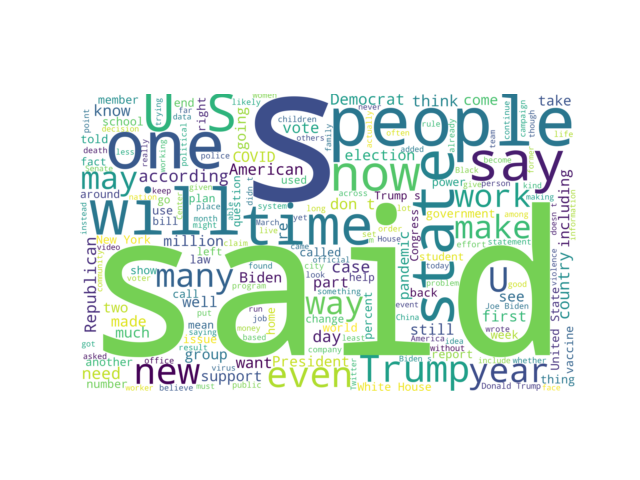
\includegraphics[width=0.9\linewidth]{figures/wordcloud_vx.png}
    \caption{Wordcloud}
    \label{fig:wordcloud}
\end{figure}


\begin{figure}[ht]
    \centering
    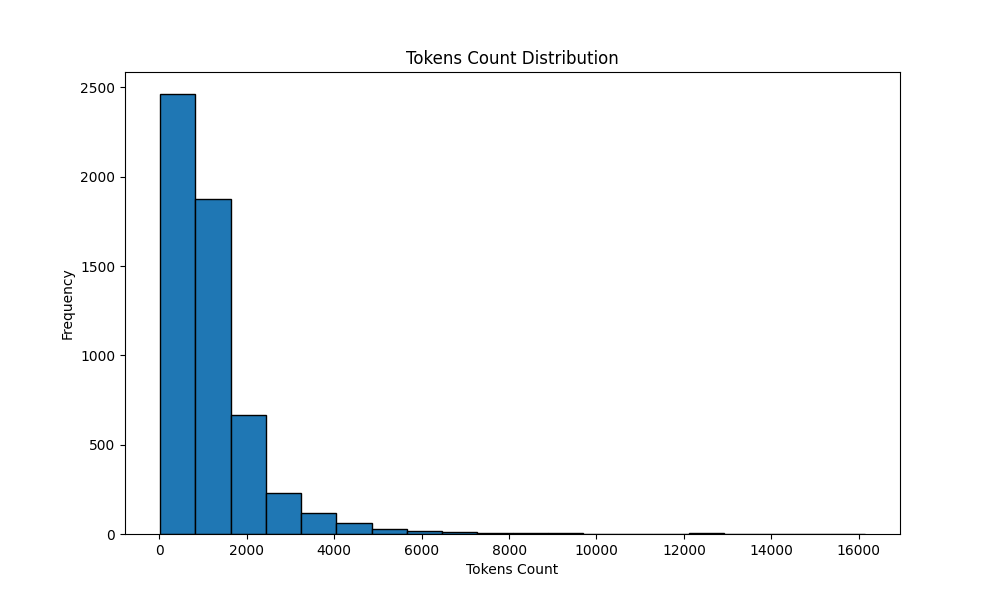
\includegraphics[width=0.9\linewidth]{figures/tokens_count_vx_hist.png}
    \caption{Tokens count distribution}
    \label{fig:tokens_hist}
\end{figure}


\begin{figure}[ht]
    \centering
    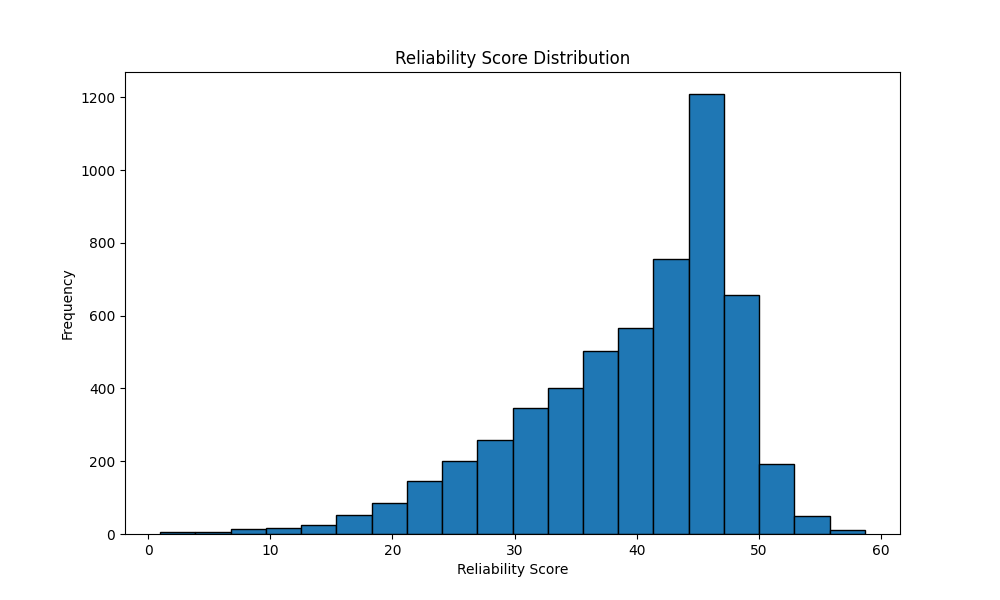
\includegraphics[width=0.9\linewidth]{figures/reliability_score_hist.png}
    \caption{Reliability score distribution}
    \label{fig:reliability_score_hist}
\end{figure}

\begin{figure}[ht]
    \centering
    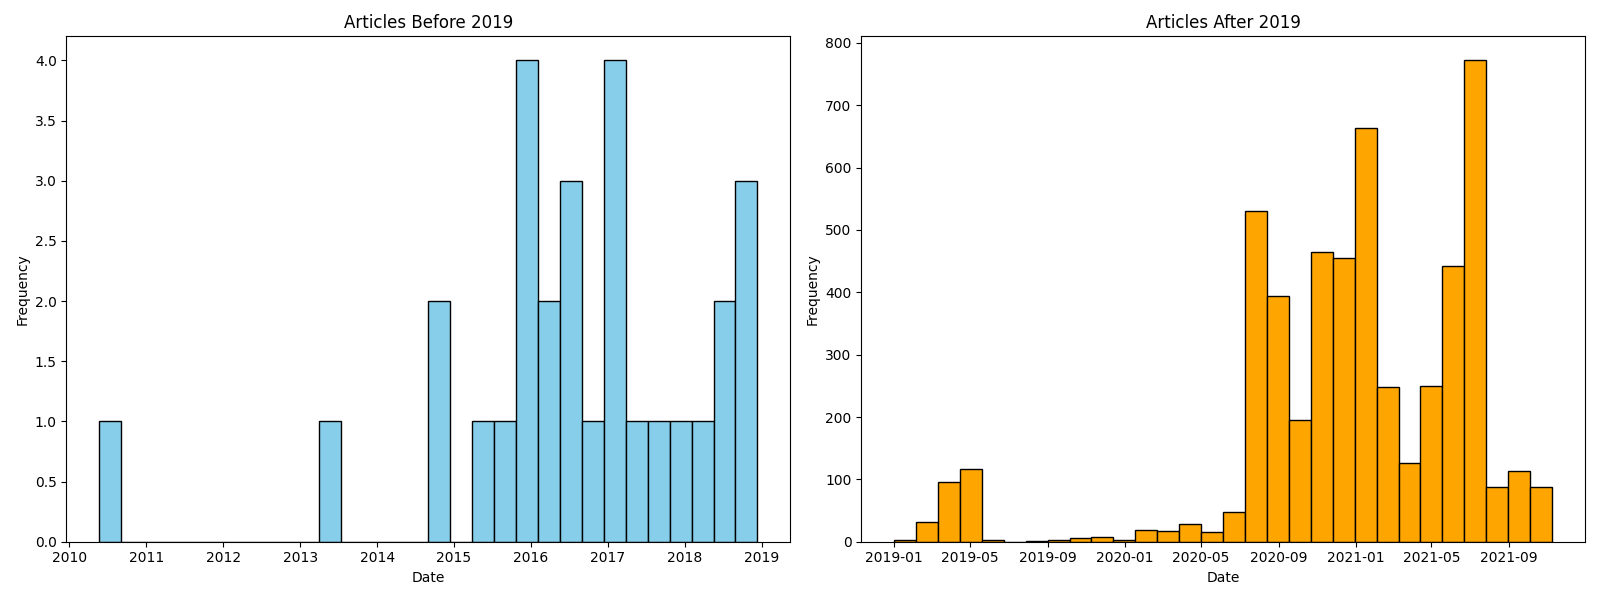
\includegraphics[width=0.9\linewidth]{figures/dates_hist.png}
    \caption{Dates distribution}
    \label{fig:dates_hist}
\end{figure}

\begin{figure}[ht]
    \centering
    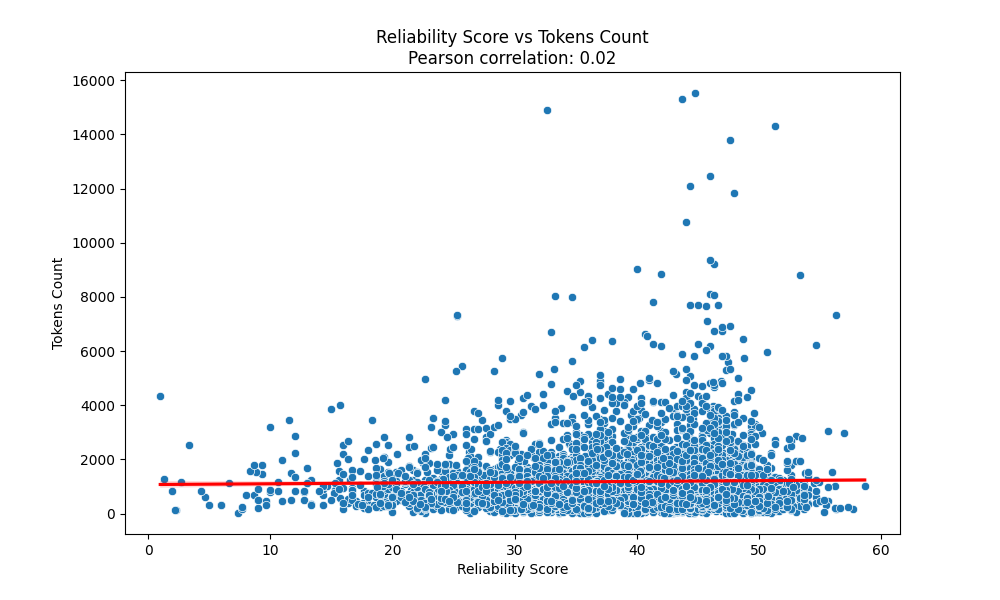
\includegraphics[width=0.9\linewidth]{figures/correlation_tokens_reliability_score.png}
    \caption{Pearson correlation between tokens count and reliability score}
    \label{fig:pearson_correlation}
\end{figure}



Further analysis (Figure \ref{fig:pearson_correlation}) shown that there is virtually no linear relationship between between tokens count and reliability score, with a Pearson correlation coefficient is 0.02. This proves that the length of an article has no significant impact with its reliability score. In other words, longer articles are not necessarily more or less reliable than shorter ones based on the provided data.

\begin{comment}
relationship between words and reliability score?
\end{comment}

\begin{comment}
Additionally, BAT includes 175,807 comments and retweets referring to the articles.

The existing literature suggests that labels provided by Ad Fontes media are suitable for media bias-related tasks and are of high quality [43]. However, especially since it relies on manual labels, the Ad Fontes article set does not cover the full range of political and non-political, recent and less recent, or controversial and non-controversial topics. The article selection by Ad Fontes media thus likely introduces bias into the dataset.

Ad Fontes: Bentley et al. (2019) (Understanding Online News Behaviors) show that the portals’ labels are highly correlated to findings from social scientists.

\end{comment}


% \section{Conclusion}
% The final section of the chapter gives an overview of the important results
% of this chapter. This implies that the introductory chapter and the
% concluding chapter don't need a conclusion.


%%% Local Variables: 
%%% mode: latex
%%% TeX-master: "thesis"
%%% End: 
